\chapter{Dust-to-Gas Ratio and $\alpha_{CO}$}

\section{Minimizing Scatter Dust-to-Gas Ratio}

In order to determine the amount of molecular hydrogen present, we have chosen to use the dust based method to determine a conversion factor.  In our analysis we have used the conversion factor $\alpha_{CO}$ which will return the amount of molecular hydrogen present in terms of its surface density.  Calculating the amour of molecular hydrogen present with this method involves reducing the scatter of the dust to gas ratio of each pixel.  The dust-to-gas ratio is calculated using

\begin{equation}\label{dgr}
  \delta_{DGR} = \frac{\Sigma_{dust}}{I_{CO}*\alpha_{CO} + \Sigma_{HI}}
\end{equation}

where $\delta_{DGR}$ is the ratio of the surface densities of the dust and gas present in the system, $\Sigma_{dust}$ is the surface density of the dust in M$_\odot$ pc$^{-2}$, $I_{CO}$ is the CO intensity in K km s$^{-1}$, $\alpha_{CO}$ is the conversion factor in units of M$_\odot$ pc$^{-2}$ (K km s$^{-1}$)$^{-1}$, and $\Sigma_{HI}$ is the surface density of the atomic hydrogen.  The scatter of the dust-to-gas ratio is determined by finding the standard deviation of the pixels assuming a Gaussian distribution.  

The ideal configuration was determined using the dust surface densities found in Chapter \ref{sed} for the Planck and Li and Draine models.  The $\alpha_{CO}$ was handled by assigning it a single value over the range of 0.01 to 100 M$_\odot$ pc$^{-2}$ (K km s$^{-1}$)$^{-1}$, and the best approximated $\alpha_{CO}$ was determined by the lowest resulting dust-to-gas scatter in the pixels of each region in Figure \ref{fig:regions}.  A 7$^{th}$ region was added that is the galaxy without the nucleus due to the lack of HI emission in the nucleus of NGC3627.  The surface density of molecular hydrogen is then determined by scaling the CO intensity by the calculated conversion factor, and the dust-to-gas ratio is then found by dividing the dust surface density by the sum of the HI and H$_2$ surface densities.  The results using Planck model with the CO J=1-0 line are shown in Figure \ref{fig:dgr_co10} where the right panel shows the ratio of H$_2$ to HI against the value of the dust-to-gas ratio in each pixel where the solid red line indicates the mean value for the dust-to-gas ratio and the dotted lines show the variance associated with the configuration.  The left panels of Figure \ref{fig:dgr_co10} show the trend of $\alpha_{CO}$ and the scatter in the dust-to-gas ratio.  The numerical values of the dust-to-gas ratio, $\alpha_{CO}$, and H$_2$ surface density using both the Planck and Li and Draine dust masses are shown in Table \ref{tab:dgr_10t}.  The error on the dust to gas ratio  in Table \ref{tab:dgr_10t} is the same as the minimum scatter found.

\begin{figure}\label{fig:dgr_co10}
  \begin{subfigure}[t]{1\textwidth}
    \centering
    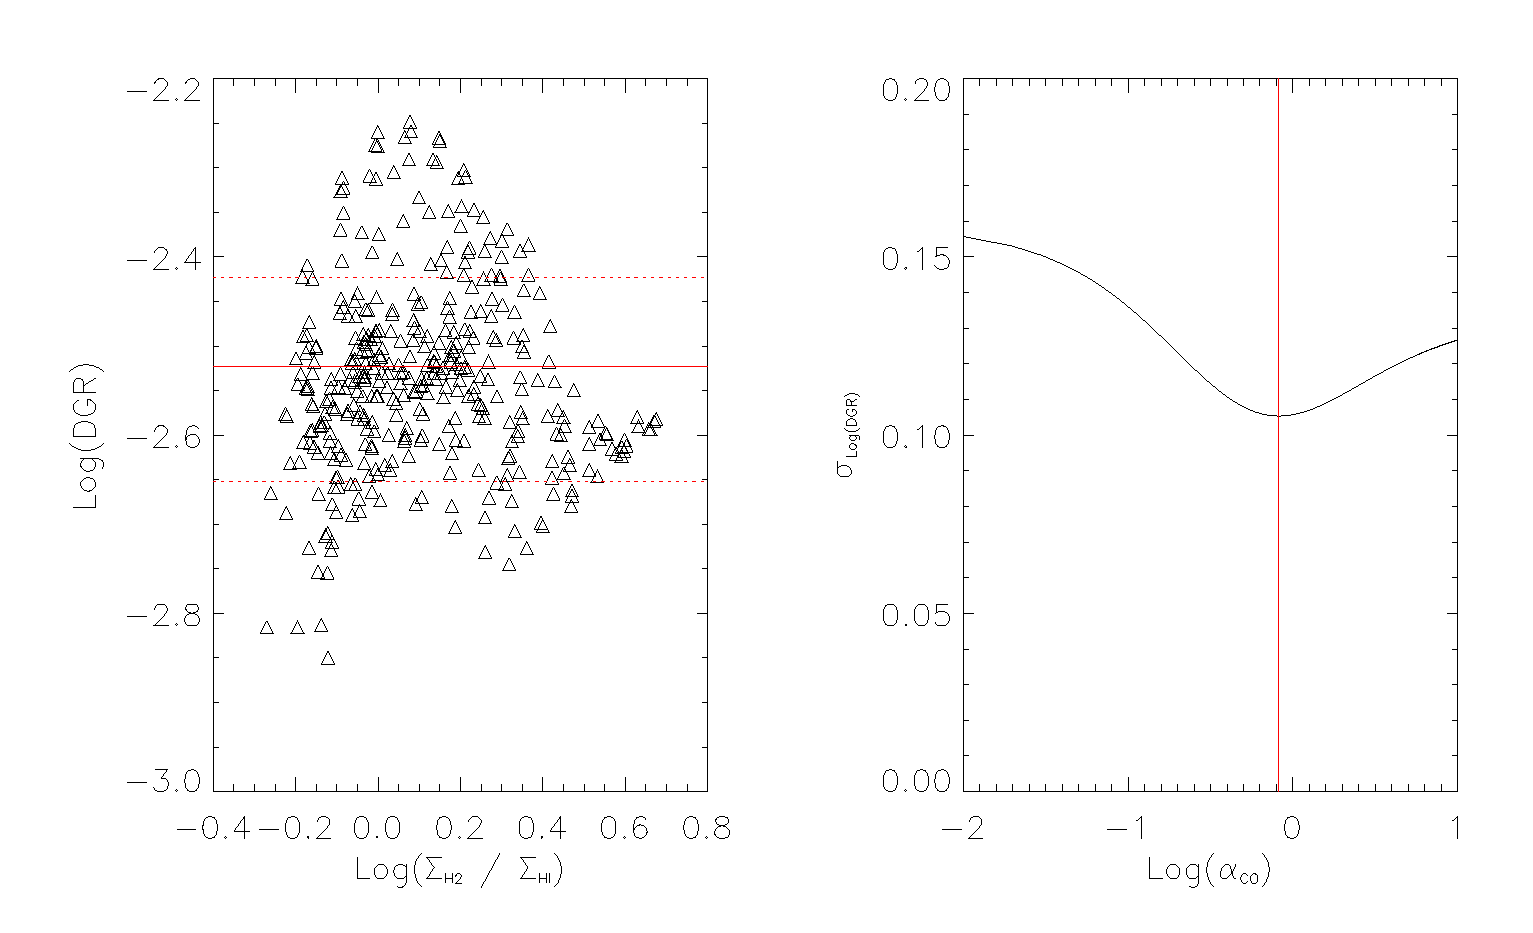
\includegraphics[width=1.\textwidth]{dgr_imgs/region_1_aco_output_10.eps}
    \caption{Region 1}
  \end{subfigure}

  \begin{subfigure}[t]{1\textwidth}
    \centering
    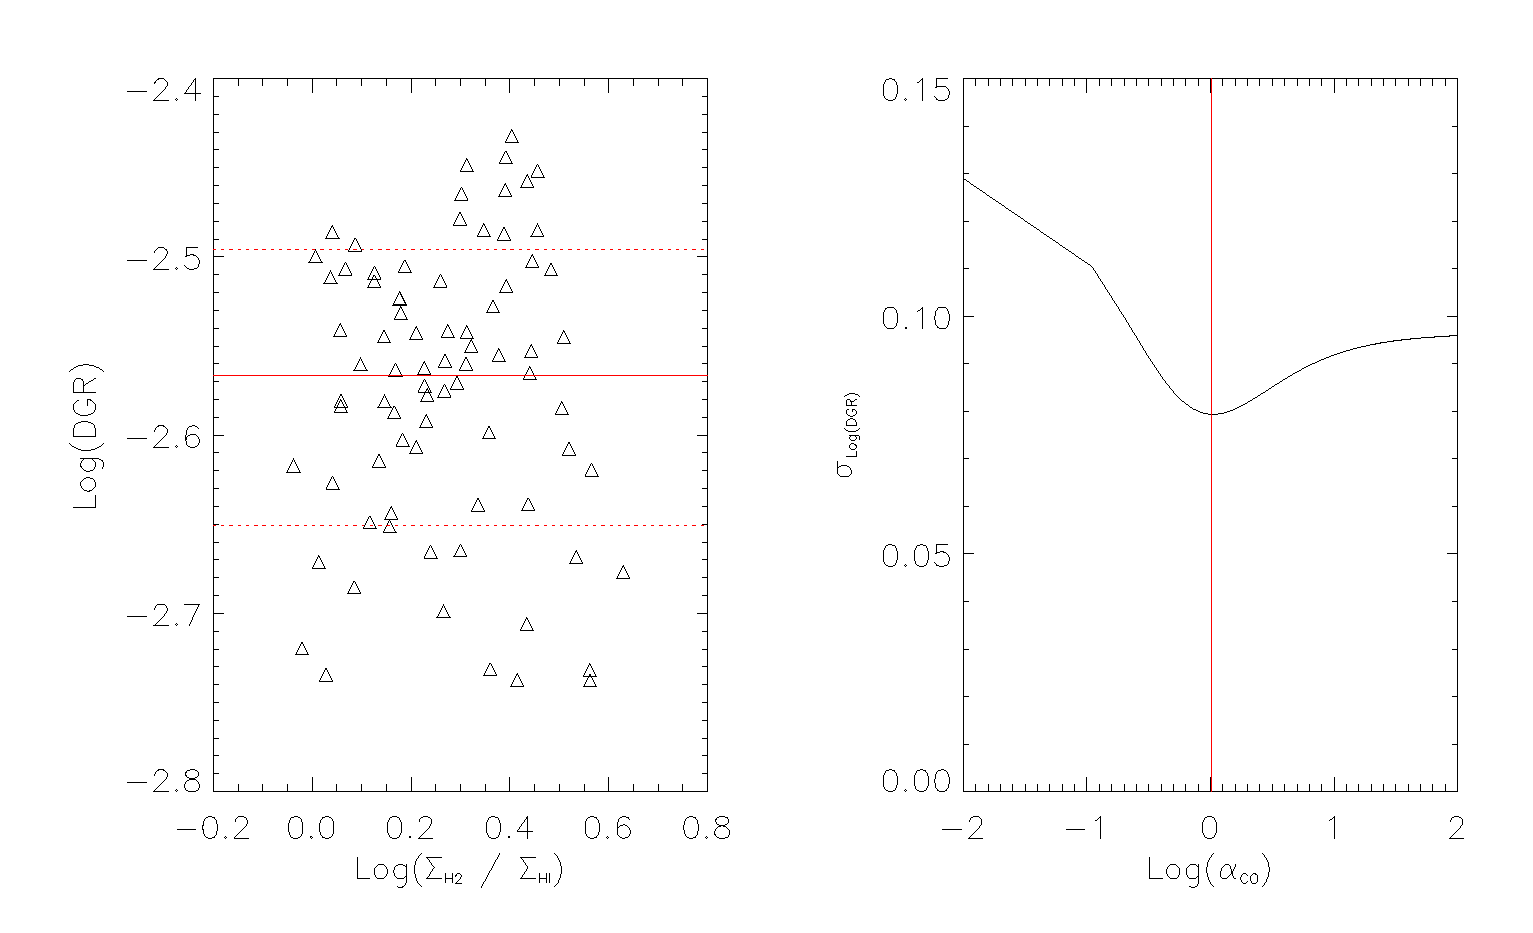
\includegraphics[width=1.\textwidth]{dgr_imgs/region_2_aco_output_10.eps}
    \caption{Region 2}
  \end{subfigure}
   \caption[Dust-to-Gas Ratio Determination Plots for CO J=1-0]{Plots of the dust-to-gas ratio vs the H$_2$ to HI surface densities using the calculated $\alpha_{CO}$ and the scatter in the dust-to-gas ratio against the $\alpha_{CO}$ values used.  Each were calculated using the CO J=1-0 line.}
   \label{fig:dgr_co10}
\end{figure}

\begin{figure}  
  \ContinuedFloat
  \begin{subfigure}[t]{1\textwidth}
    \centering
    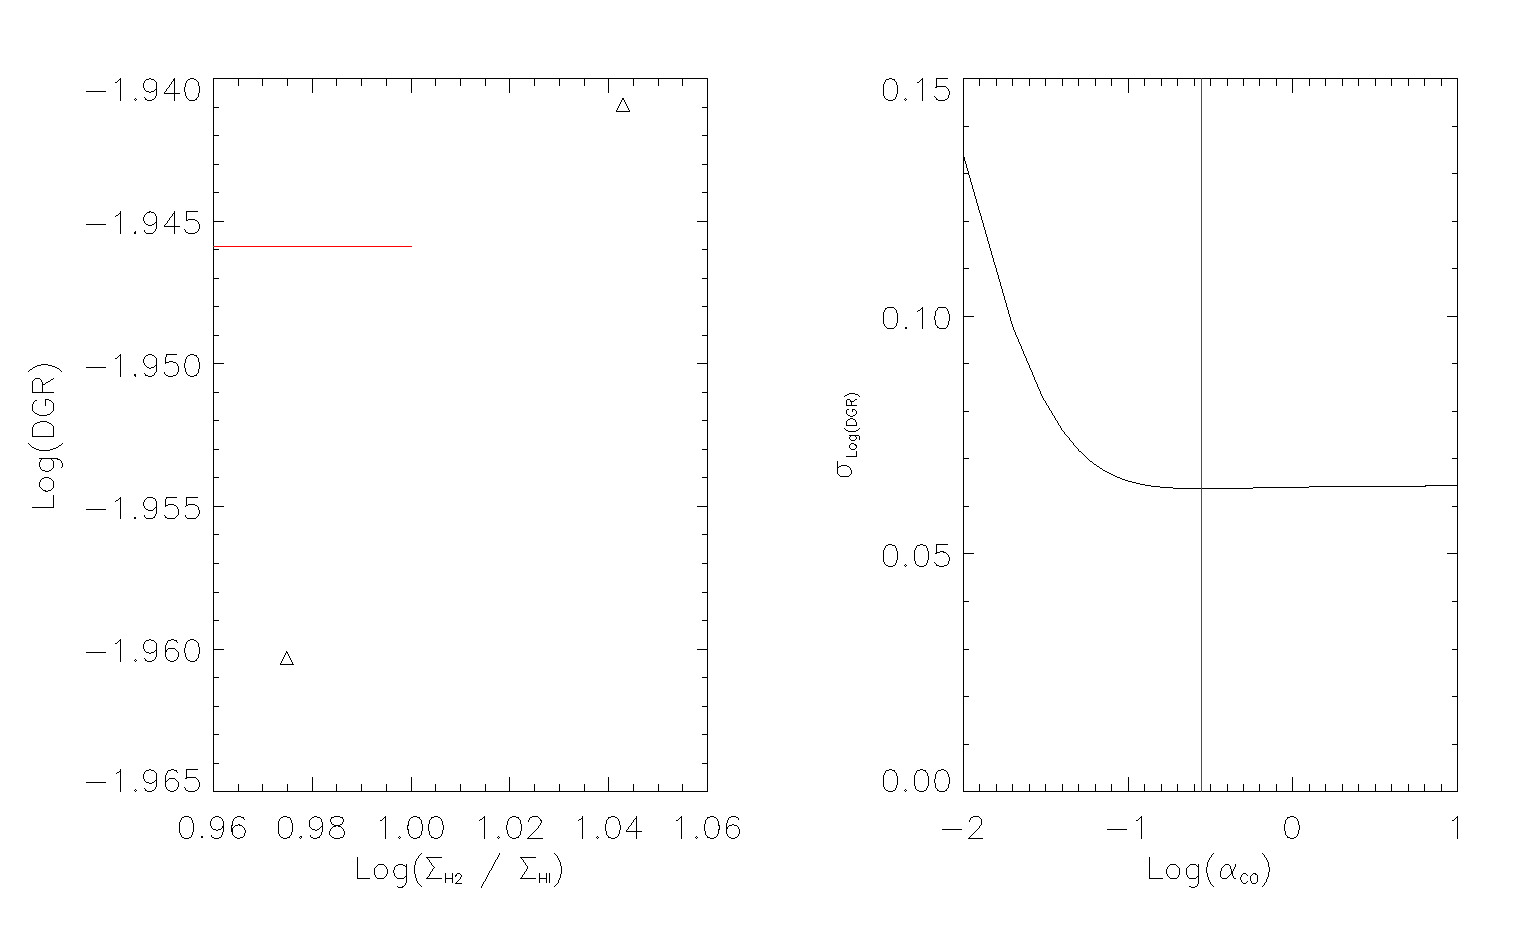
\includegraphics[width=1.\textwidth]{dgr_imgs/region_3_aco_output_10.eps}
    \caption{Region 3}
  \end{subfigure}

  \begin{subfigure}[t]{1\textwidth}
    \centering
    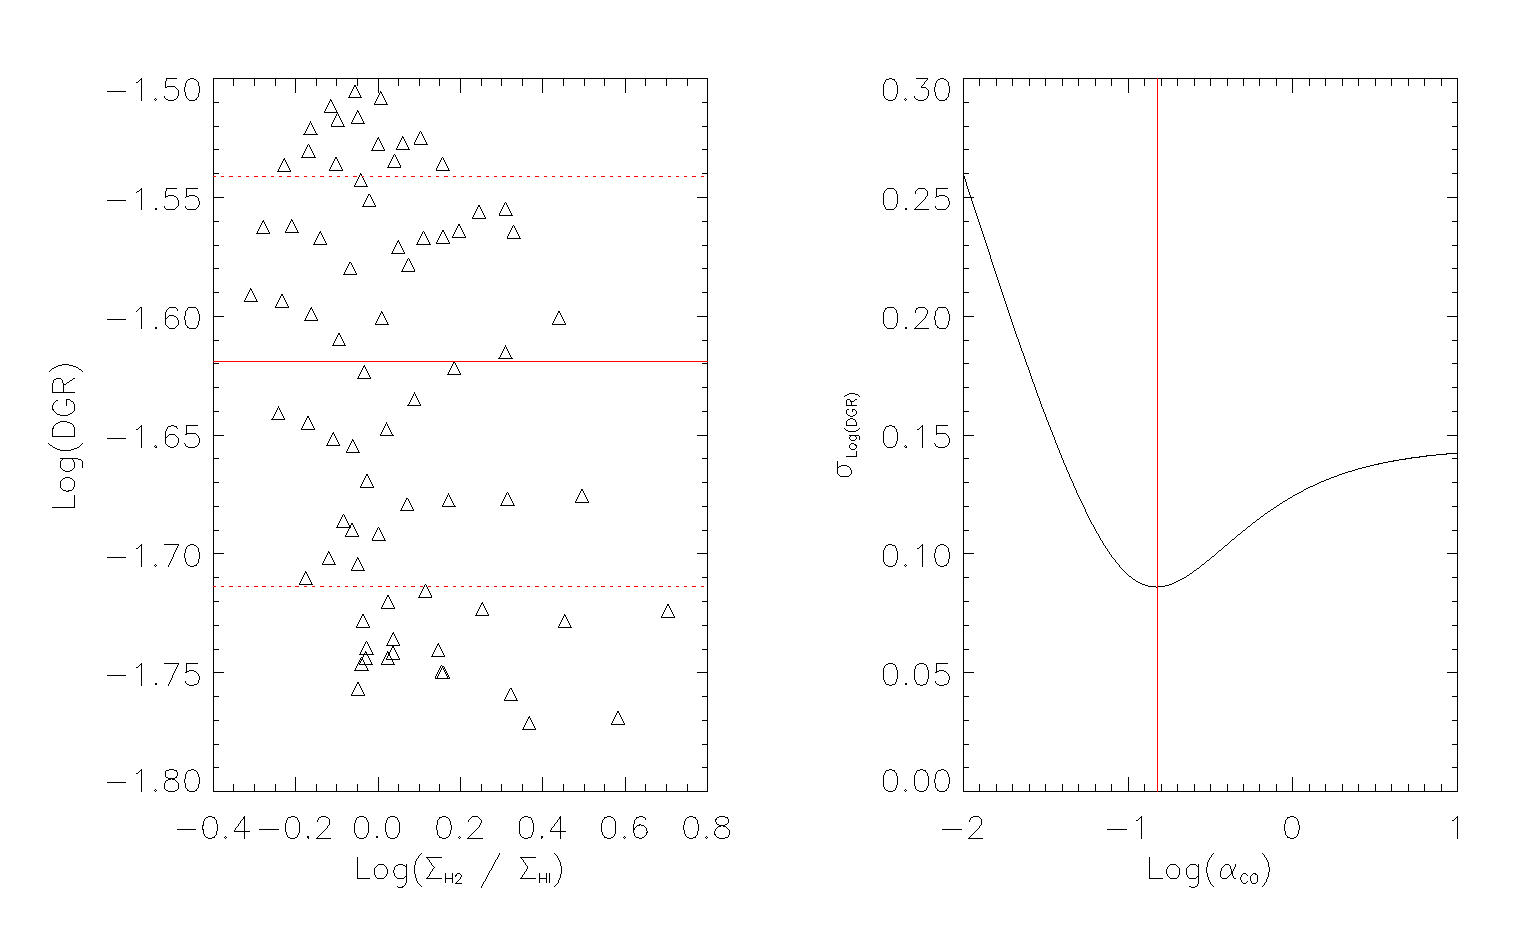
\includegraphics[width=1.\textwidth]{dgr_imgs/region_4_aco_output_10.eps}
    \caption{Region 4}
  \end{subfigure}
   \caption[Dust-to-Gas Ratio Determination Plots for CO J=1-0]{Plots of the dust-to-gas ratio vs the H$_2$ to HI surface densities using the calculated $\alpha_{CO}$ and the scatter in the dust-to-gas ratio against the $\alpha_{CO}$ values used.  Each were calculated using the CO J=1-0 line.}
   \label{fig:dgr_co10}
\end{figure}

\begin{figure}
  \ContinuedFloat
  \begin{subfigure}[t]{1\textwidth}
    \centering
    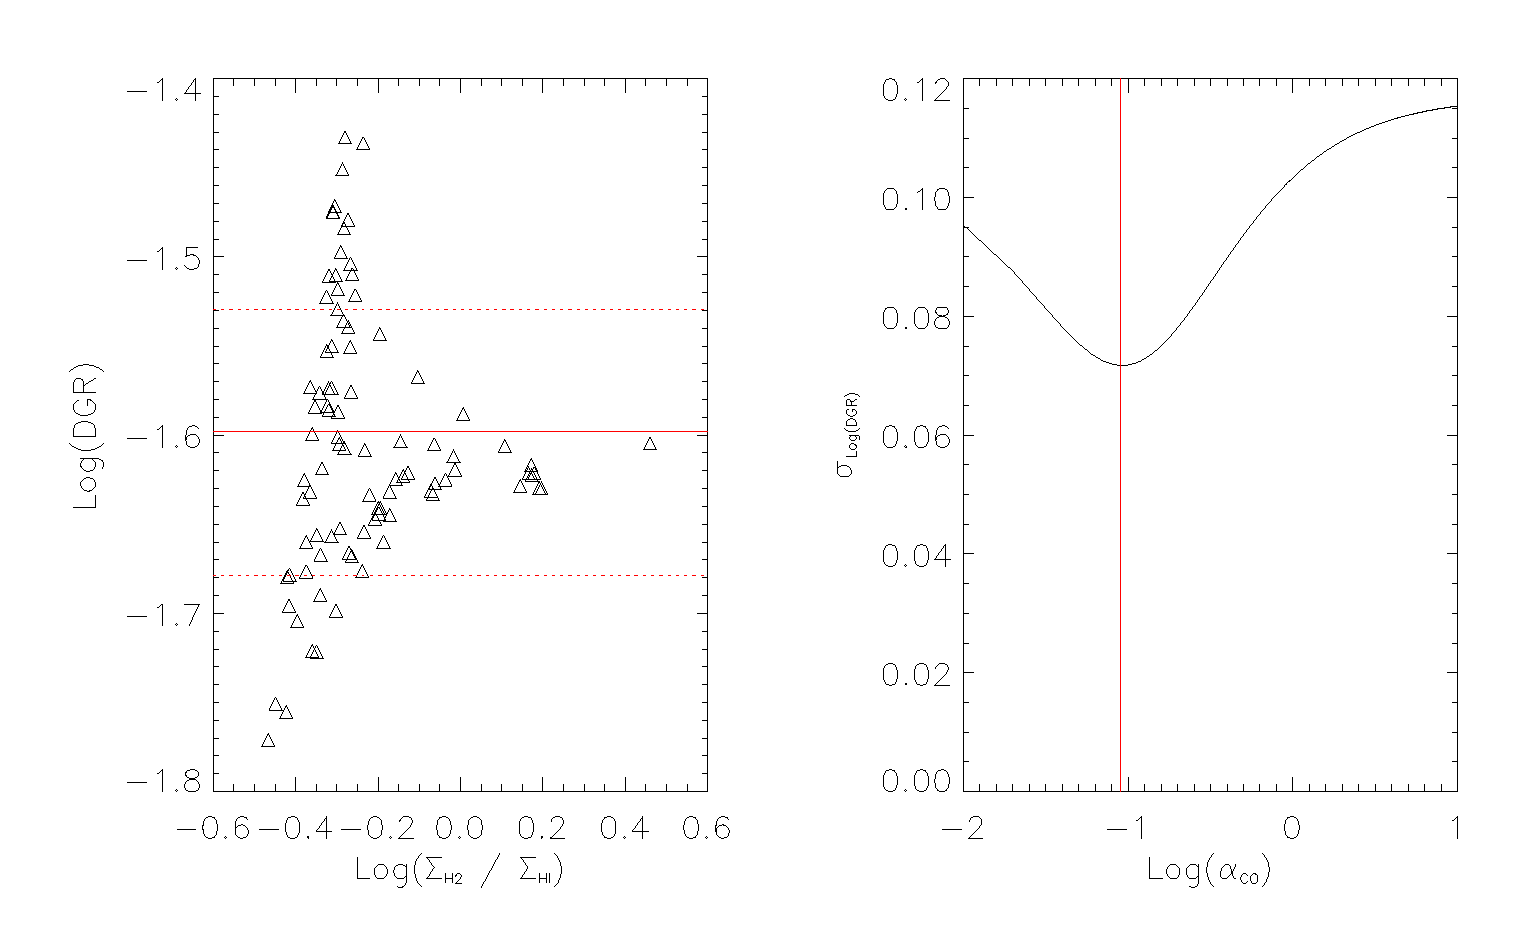
\includegraphics[width=1.\textwidth]{dgr_imgs/region_5_aco_output_10.eps}
    \caption{Region 5}
  \end{subfigure}

  \begin{subfigure}[t]{1\textwidth}
    \centering
    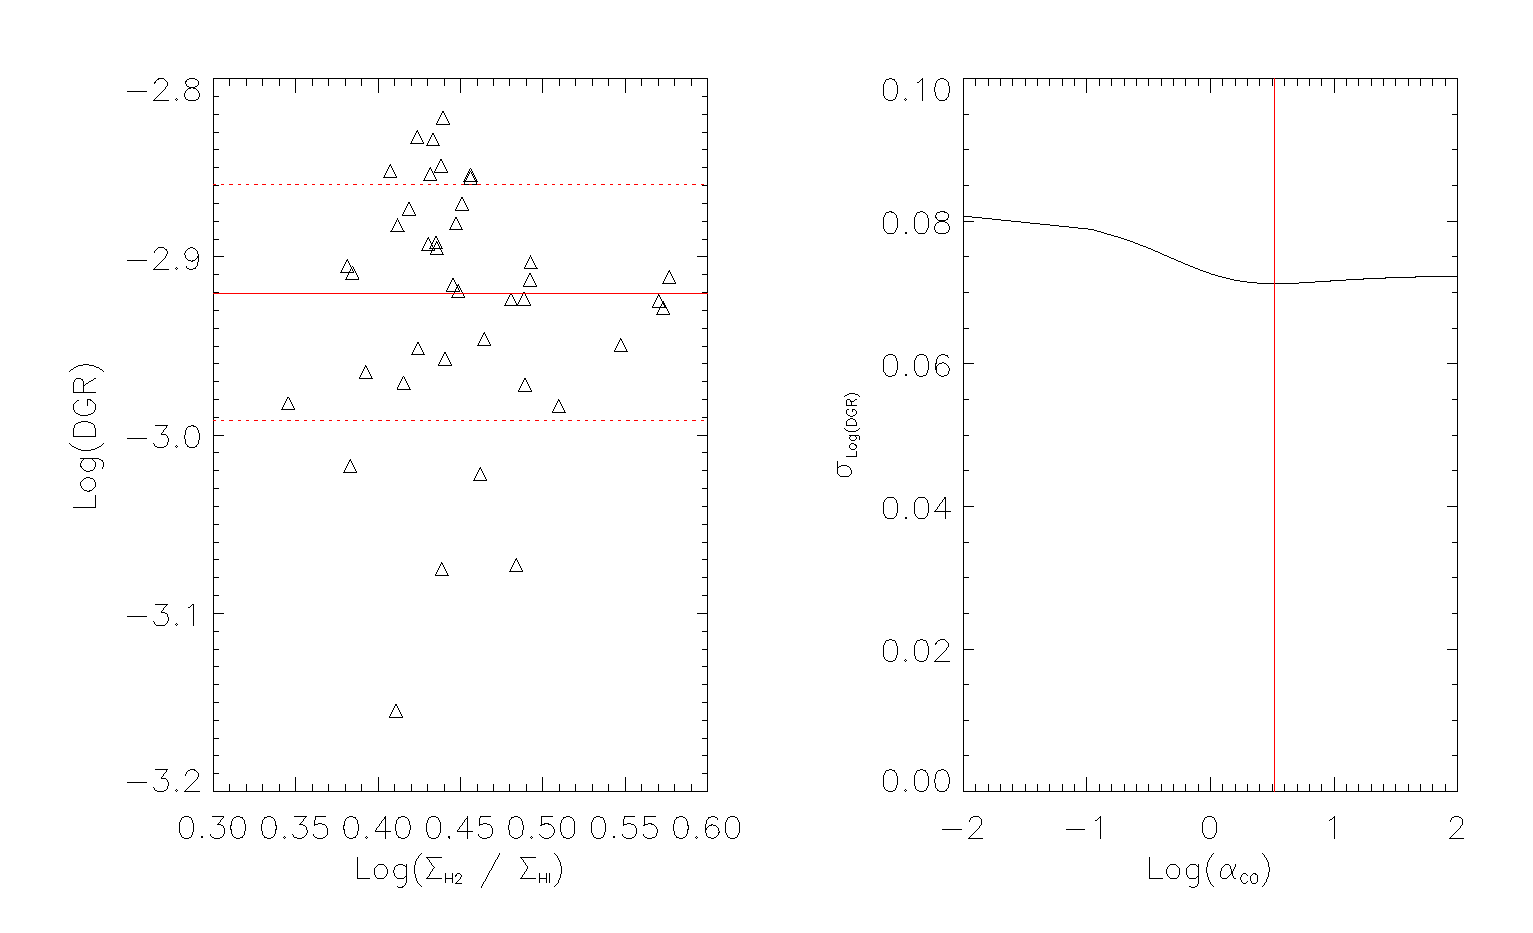
\includegraphics[width=1.\textwidth]{dgr_imgs/region_6_aco_output_10.eps}
    \caption{Region 6}
  \end{subfigure}
   \caption[Dust-to-Gas Ratio Determination Plots for CO J=1-0]{Plots of the dust-to-gas ratio vs the H$_2$ to HI surface densities using the calculated $\alpha_{CO}$ and the scatter in the dust-to-gas ratio against the $\alpha_{CO}$ values used.  Each were calculated using the CO J=1-0 line.}
   \label{fig:dgr_co10}
\end{figure}

\begin{figure}
  \ContinuedFloat
  \begin{subfigure}[t]{1\textwidth}
    \centering
    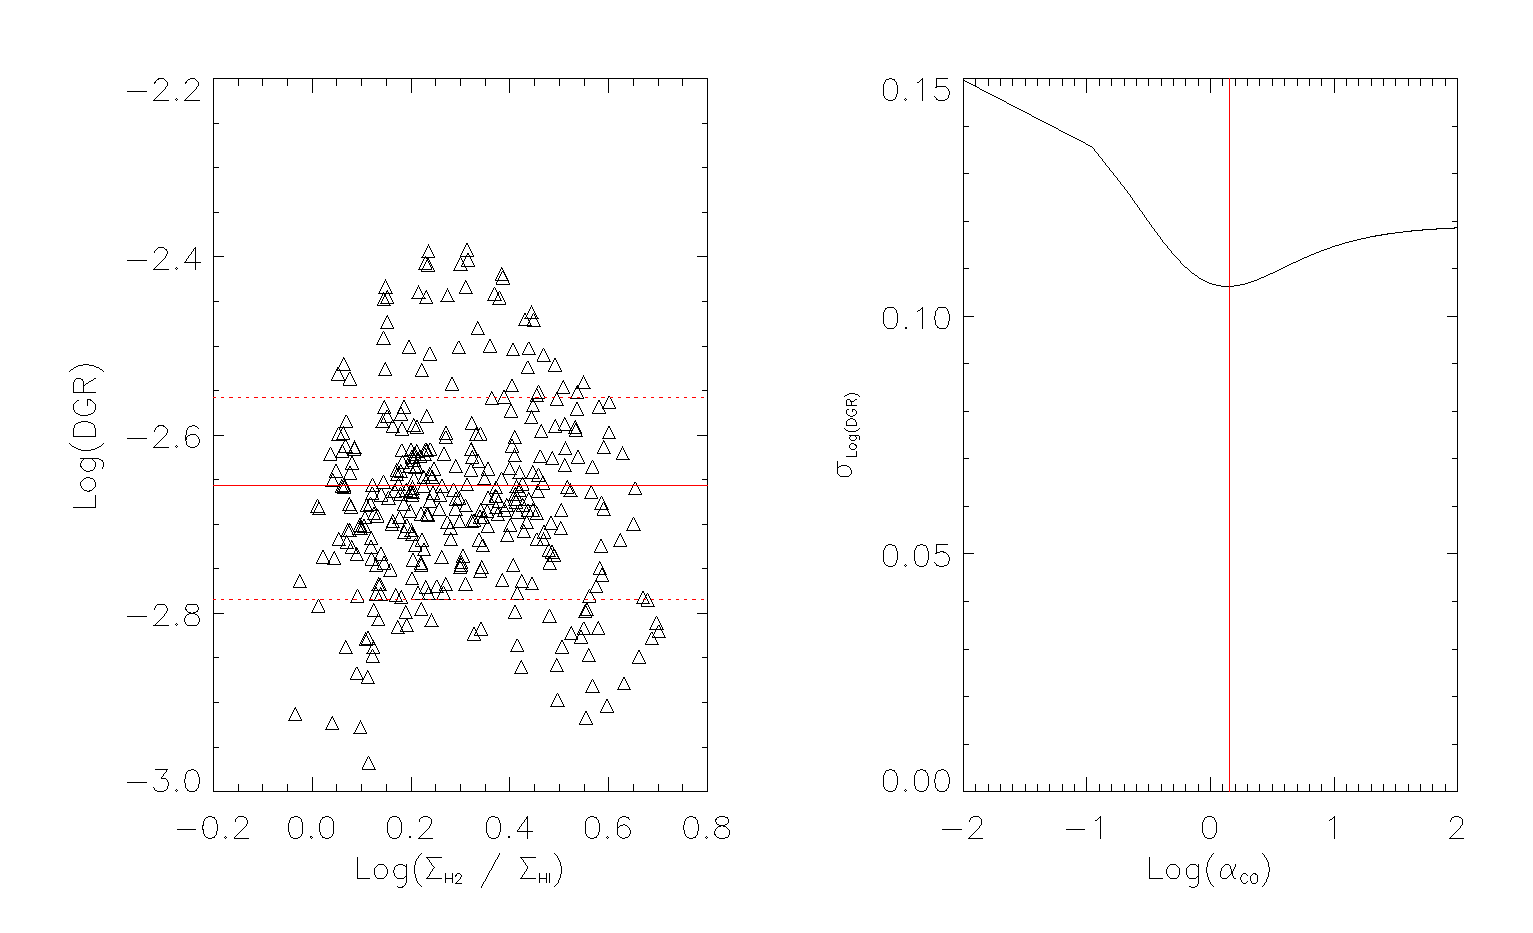
\includegraphics[width=1.\textwidth]{dgr_imgs/region_1-3_aco_output_10.eps}
    \caption{Region 1 Without the Nucleus}
  \end{subfigure}
  \caption[Dust-to-Gas Ratio Determination Plots for CO J=1-0]{Plots of the dust-to-gas ratio vs the H$_2$ to HI surface densities using the calculated $\alpha_{CO}$ and the scatter in the dust-to-gas ratio against the $\alpha_{CO}$ values used.  Each were calculated using the CO J=1-0 line.}
   \label{fig:dgr_co10}
\end{figure}

\begin{deluxetable}{rccc}
  \tabletypesize{\footnotesize}
  \tablecolumns{4}
  \tablewidth{0pt}
  \tablecaption{Dust-to-gas ratio, $\alpha_{CO}$, and H$_2$ Surface Density using CO J=1-0 Tracer\label{tab:dgr_10t}}
  \tablehead{
    \colhead{Opacity Model} &
    \colhead{Dust-to-Gas Ratio} &
    \colhead{$\alpha_{CO}$} &
    \colhead{Average $\Sigma_{H_2}$ per Pixel} \\
    &
    &
    [M$_\odot$ pc$^{-2}$ (K km s$^{-1}$)$^{-1}$] &
    [M$_\odot$ pc$^{-2}$] }
  \startdata
    \sidehead{Region 1}
      Planck &        0.021 $\pm$ 0.005 & 0.150 $\pm$ 0.005 & 3 $\pm$ 2 \\
      Li and Draine & 0.09  $\pm$ 0.02  & 0.160 $\pm$ 0.005 & 3 $\pm$ 2 \\
    \sidehead{Region 2}
      Planck &        0.013 $\pm$ 0.003 & 0.290 $\pm$ 0.005 & 7 $\pm$ 3 \\
      Li and Draine & 0.05  $\pm$ 0.01  & 0.310 $\pm$ 0.005 & 8 $\pm$ 3 \\
    \sidehead{Region 3}
      Planck &        0.038 $\pm$ 0.004 & 0.070 $\pm$ 0.005 & 2.6 $\pm$ 0.6\\
      Li and Draine & 0.17  $\pm$ 0.02  & 0.070 $\pm$ 0.005 & 2.6 $\pm$ 0.6\\
    \sidehead{Region 4}
      Planck &        0.028 $\pm$ 0.005 & 0.110 $\pm$ 0.005 & 3 $\pm$ 1 \\
      Li and Draine & 0.12  $\pm$ 0.02  & 0.110 $\pm$ 0.005 & 3 $\pm$ 1 \\
    \sidehead{Region 5}
      Planck &        0.025 $\pm$ 0.004 & 0.090 $\pm$ 0.005 & 1.2 $\pm$ 0.6\\
      Li and Draine & 0.11  $\pm$ 0.02  & 0.100 $\pm$ 0.005 & 1.4 $\pm$ 0.6\\
    \sidehead{Region 6}
      Planck &        0.009 $\pm$ 0.001 & 0.590 $\pm$ 0.005 & 6 $\pm$ 1 \\
      Li and Draine & 0.040 $\pm$ 0.006 & 0.610 $\pm$ 0.005 & 6 $\pm$ 1 \\
    \sidehead{No Nucleus}
      Planck &        0.019 $\pm$ 0.004 & 0.180 $\pm$ 0.005 & 3 $\pm$ 2 \\
      Li and Draine & 0.08  $\pm$ 0.02  & 0.190 $\pm$ 0.005 & 3 $\pm$ 2 \\
  \enddata
\end{deluxetable}

While CO J=1-0 is the standard molecular tracer of H$_2$ \citep{bolatto2013}, the observations are not always available.  In the situation without CO J=1-0 data an alternative excitation state of CO is used.  This was done by \cite{sandstrom2013} using the CO J=2-1 transition, and by \cite{warren2010} using the CO J=3-2 transition, where the observations were scaled to the expected intensity of the CO J=1-0 using a line ratio.  We have found the line ratio of the 2-1/1-0 to be 0.39 for the galaxy on a whole, and can examine the effects of using this technique to approximate the CO J=1-0 transition in this method.  The results for the dust-to-gas ratio, $\alpha_{CO}$, and H$_2$ surface density are shown in Table \ref{tab:dgr_21}.

\begin{deluxetable}{rccc}
  \tabletypesize{\footnotesize}
  \tablecolumns{4}
  \tablewidth{0pt}
  \tablecaption{Dust-to-gas ratio, $\alpha_{CO}$, and H$_2$ Surface Density using CO J=2-1 Tracer\label{tab:dgr_21}}
  \tablehead{
    \colhead{Opacity Model} &
    \colhead{Dust-to-Gas Ratio} &
    \colhead{$\alpha_{CO}$} &
    \colhead{Average $\Sigma_{H_2}$ per Pixel} \\
    &
    &
    [M$_\odot$ pc$^{-2}$ (K km s$^{-1}$)$^{-1}$] &
    [M$_\odot$ pc$^{-2}$] }
  \startdata
    \sidehead{Region 1}
      Planck &        0.016  $\pm$ 0.002  & 0.630 $\pm$ 0.005 & 5   $\pm$ 3 \\
      Li and Draine & 0.07   $\pm$ 0.01   & 0.670 $\pm$ 0.005 & 5   $\pm$ 3 \\
    \sidehead{Region 2} 
      Planck &        0.0147 $\pm$ 0.007  & 0.650 $\pm$ 0.005 & 6   $\pm$ 3 \\
      Li and Draine & 0.063  $\pm$ 0.003  & 0.680 $\pm$ 0.005 & 7   $\pm$ 3 \\
    \sidehead{Region 3}
      Planck &        0.049  $\pm$ 0.005  & 0.150 $\pm$ 0.005 & 1.9 $\pm$ 0.5 \\
      Li and Draine & 0.21   $\pm$ 0.02   & 0.160 $\pm$ 0.005 & 2.0 $\pm$ 0.6 \\
    \sidehead{Region 4}
      Planck &        0.011  $\pm$ 0.001  & 1.020 $\pm$ 0.005 & 12  $\pm$ 4 \\
      Li and Draine & 0.045  $\pm$ 0.005  & 1.060 $\pm$ 0.005 & 12  $\pm$ 4 \\
    \sidehead{Region 5}
      Planck &        0.013  $\pm$ 0.002  & 0.880 $\pm$ 0.005 & 4  $\pm$ 1\\
      Li and Draine & 0.054  $\pm$ 0.008  & 0.930 $\pm$ 0.005 & 5  $\pm$ 2\\
    \sidehead{Region 6}
      Planck &        0.0109 $\pm$ 0.0008 & 1.140 $\pm$ 0.005 & 4  $\pm$ 1 \\
      Li and Draine & 0.046  $\pm$ 0.004  & 1.180 $\pm$ 0.005 & 5  $\pm$ 1 \\
    \sidehead{No Nucleus}
      Planck &        0.013  $\pm$ 0.002  & 0.830 $\pm$ 0.005 & 6  $\pm$ 4 \\
      Li and Draine & 0.055  $\pm$ 0.008  & 0.880 $\pm$ 0.005 & 6  $\pm$ 4 \\
  \enddata
\end{deluxetable}

\section{Effects of the Dust Model and CO Treatment}

The effects of the dust model are mainly seen in the dust-to-gas ratio for the CO J=1-0 emission.  Since the major difference in the two models was the outputted mass, this would make sense to see the Li and Draine model produce larger dust-to-gas ratios.  The conversion factors show some decrease, but the over all molecular gas surface density all agree within error for each region.  The same trend of larger dust-to-gas ratios are seen when scaling the CO J=2-1 emission the dust-to-gas ratio of the Planck model is larger than the Li and Draine model, however the galaxy as a whole and regions 5 and 6 also show a larger $\alpha_{CO}$ which increases the average surface density of those regions.
  
The effect of the CO treatment shows the same trend trend with the dust models showing that the Li and Draine model yields a higher dust-to-gas ratio, but using the CO J=2-1 emission with a 2-1/1-0 ratio applied significantly increases the conversion factor for each region by a factor of  2 to 10.  Despite the increase in $\alpha_{CO}$ we still see the same masses for all of the regions except for regions 4 and 5.  The conflicting surface densities are due to the behavior of the 2-1/1-0 ratio in these regions.  Region 5 displays a large gradient in 2-1/1-0 ratio as you move south along the spiral arm, and the 75\% percent decrease in region 4 is due to the entire region's 2-1/1-0 ratio is nearly double the mean value of the galaxy.

\section{Validity of Results}

If NGC3627 were to show Milky Way like values, we would expect $\alpha_{CO}\approx$4 \citep{sandstrom2013}.  Except the $\alpha_{CO}$ values given for the the CO J=2-1 emission suggest  NGC3627 is similar to U/LIRG type galaxies whose $\alpha_{CO}$ range has been given as 0.3 - 1.3 M$_\odot$ pc$^{-2}$ (K km s$^{-1}$)$^{-1}$ \citep{downes1998}, and the CO J=1-0 emission falls below the U/LIRG range.  Even our smallest dust-to-gas ratio falls above the typical values found in late type galaxies of 0.005 - 0.01 \citep{smith2012}.  If we compare our results to values recently calculated using the same method by \cite{sandstrom2013}, we find that our conversion factor is much lower than their average of 1.2 M$_\odot$ pc$^{-2}$ (K km s$^{-1}$)$^{-1}$, and our dust-to-gas ratio is much larger than their average of $\approx$0.017.  The low $\alpha_{CO}$ and high dust-to-gas ratios are due mainly to the filtering process applied to our data ($\S$ \ref{ancillary}), in particular the amount of HI removed from the filtering.  If we follow the steps taken in \cite{sandstrom2013} by using the Li and Draine dust model with the CO J=2-1 emission such that none of the gas has been filtered, we get the results shown in Table \ref{tab:no_filt}.

\begin{deluxetable}{cccc}
  \tabletypesize{\footnotesize}
  \tablecolumns{4}
  \tablewidth{0pt}
  \tablecaption{Dust-to-gas ratio, $\alpha_{CO}$, and H$_2$ Surface Density using CO J=2-1 Tracer with no Emission Filtering \label{tab:no_filt}}
  \tablehead{
    \colhead{Region} &
    \colhead{Dust-to-Gas Ratio} &
    \colhead{$\alpha_{CO}$} &
    \colhead{Average $\Sigma_{H_2}$ per Pixel} \\
    &
    &
    [M$_\odot$ pc$^{-2}$ (K km s$^{-1}$)$^{-1}$] &
    [M$_\odot$ pc$^{-2}$] }
  \startdata
      1 & 0.010   $\pm$ 0.001   & 3.890 $\pm$ 0.005 & 31 $\pm$ 18 \\
      2 & 0.0107  $\pm$ 0.0009  & 3.470 $\pm$ 0.005 & 36 $\pm$ 15 \\
      3 & 0.0174  $\pm$ 0.0009  & 1.380 $\pm$ 0.005 & 19 $\pm$ 5  \\
      4 & 0.013   $\pm$ 0.001   & 3.000 $\pm$ 0.005 & 36 $\pm$ 12 \\
      5 & 0.0085  $\pm$ 0.0009  & 5.080 $\pm$ 0.005 & 28 $\pm$ 9  \\
      6 & 0.0065  $\pm$ 0.0007  & 7.930 $\pm$ 0.005 & 35 $\pm$ 10 \\
      No Nucleus & 0.0076  $\pm$ 0.0009  & 5.780 $\pm$ 0.005 & 44 $\pm$ 25 \\
  \enddata
\end{deluxetable}
 
